\documentclass[a4paper, 12pt]{article}
\usepackage[a4paper,top=1.5cm, bottom=1.5cm, left=1cm, right=1cm]{geometry}
\usepackage{cmap}					
\usepackage{mathtext} 				
\usepackage[T2A]{fontenc}			
\usepackage[utf8]{inputenc}			
\usepackage[english,russian]{babel}
\usepackage{multirow}
\usepackage{graphicx}
\usepackage{wrapfig}
\usepackage{tabularx}
\usepackage{float}
\usepackage{longtable}
\usepackage{hyperref}
\hypersetup{colorlinks=true,urlcolor=blue}
\usepackage[rgb]{xcolor}
\usepackage{amsmath,amsfonts,amssymb,amsthm,mathtools} 
\usepackage{icomma} 
\usepackage{euscript}
\usepackage{mathrsfs}
\usepackage{enumerate}
\usepackage{caption}
\usepackage{enumerate}
\usepackage{graphicx}
\usepackage{caption}
\usepackage{subcaption}

\usepackage[europeanresistors, americaninductors]{circuitikz}
\DeclareMathOperator{\sgn}{\mathop{sgn}}
\newcommand*{\hm}[1]{#1\nobreak\discretionary{}
	{\hbox{$\mathsurround=0pt #1$}}{}}


\title{\textbf{Измерение иннтенсивности радиационного фона (1.1.4)}}
\author{Павлушкин Вячеслав}
\date{Сентябрь 2021}




\begin{document}
	
	\maketitle
	
	\section{Введение}
	
	\textbf{Цель работы:} применение методов обработки экспериментальных данных для изучения статистических закономерностей при измерении интенсивности радиационного фона.
	\bigskip\\
	\textbf{Оборудование:} счетчик Гейгера-Мюллера (CTC-6), блок питания, компьютер с интерфейсом связи со счетчиком.
	
	\section{Теоретические сведения}
	
	В данной работе измеряется число частиц, проходящих через счетчик за 10 секунд, с помощью которого мы можем найти и количество за 40 секунд. Такие времена выбраны для того, чтобы продемонстрировать то, что при большем времени лучше выполняется нормальное распределение измеряемых величин и гистограмма более симметрична, чем при малых временах, когда при оработке лучше воспользоваться законом Пуассона.
	
	Если случайные события, такие как регистрация частицы счётчиком, однородны во времени и являются независимыми, то результаты их измерений подчиняются распределению Пуассона. Теория вероятности гласит, что в таком случае среднеквадратичная ошибка числа отсчётов, измеренного за некоторый интервал времени, равна квадратному корню из среднего числа отсчётов за тот же интервал:
	
	\begin{equation}
		\sigma = \sqrt{n_0}
	\end{equation}
	 
	
	При проведении многочисленных опытов за $n_0$ принимается среднее арифметическое всех результатов $\overline n$, а стандартная ошибка отклонения $\overline n$ от $n_0$ может быть вычислена по формуле:
	\[ \sigma_{\overline n} = \frac{1}{N} \sqrt{\sum_{i=1}^N(n_i - \overline n)^2}, \] где $N$ - количество измерений, $n_i$ - результат $i$-того измерения. Относительная же погрешность составит: \[ \varepsilon_{\overline n} = \frac{1}{\sqrt{\overline n N}}. \] 
	
	\begin{center}
		\textbf{Распределение Пуассона.}
	\end{center}

	Рассмотрим счетчик, регистрирующий частицы. Найдем вероятность того, что при плостности излучения $\nu$ счетчик сработает $n$ раз за время измерения. Для простоты будем считать, что счетчик обладает единичной площадью.
	
	Представим себе большое число совершенно одинаковых одновременно работающих счетчиков. Обозначимполное число счетчиков буквой $N$. Через них в секунду в среднем проходит $N\nu$ частиц, а за $dt$ пройдет $N\nu dt$ частиц. Если $dt$ достаточно мало, то за это время ни через один счетчик не пройдет двух частиц. Число счетчиков, через которые прошла частица равно $N\nu dt$, а их доля по отношению к общему числу счетчиков: $N\nu dt/N = \nu dt$. Вероятность того, что за время $dt$ через счетчик пройдет частица, равна $\nu dt$.
	
	Вычислим теперь вероятность $P_0(t)$ того, что за время $t$ через счетсик не пройдет ни одной частицы. Количество таких счетчиков в момент $t$ составляет $NP_0 (t)$, а в момент времени $t+dt$ равно $NP_0 (t+dt)$. Это число меньше, чем $NP_0 (t)$, потому что за время $dt$ их сисло убавится на $NP_0 (t)\nu dt$. Поэтому: \[NP_0 (t+dt) = NP_0(t) - NP_0 (t)\nu dt,\] \[P_0 (t+dt) = P_0(t) - P_0 (t)\nu dt.\] Разделиы это равенство на $dt$ и переходя к пределу, получим \[ \frac{dP_0}{dt} = -\nu P_0 \]  Интегрируя, найдем: 
	
	\begin{equation}
		P_0 (t) = e^{-\nu t}
		\label{puas}
	\end{equation}
	
	Вычислим теперь $P_n (t+dt)$ -- вероятность того, что за время $t+dt$ через счетчик пройдет ровно $n$ частиц. число таких счетчиков $NP_n(t+dt)$ состоит из двух частей. Первая часть -- счетчики через которые все частицы прошли за $t$ -- $NP_n(t)(1-\nu dt)$, а вторая -- счетчики, через которые за время $t$ прошло $n-1$ частиц, а последня последняя за время $dt$, их число: $NP_{n-1}(t)\nu dt$. Имеем, следовательно: \[NP_n(t+dt) = NP_n(t)(1-\nu dt) + NP_{n-1}(t)\nu dt.\]
	Разделив на $Ndt$ получаем:\[ \frac{dP_n}{dt} + \nu P_n = \nu P_{n-1}. \]
	Применяя формулу полученную реккурентности, с помощью (\ref{puas}) найдем: \[ P_n = \frac{(\nu t)^n}{n!}e^{-\nu t} \] 
	Заметим теперь, что $\nu t $, которое мы обозначим через $n_0$, равно среднему числу частиц, проходящих через счетчик за время $t$. Формула примет вид:
	
	\begin{equation}
		P_n = \frac{n_0^n}{n!}e^{-\nu t}
	\end{equation}
	
	\section{Ход работы}
	
	\begin{enumerate}
		\item Включаем компьютер и счетчик Гейгера-Мюллера. Начинается основной эксперимент.
		\item Проводим демонстрационный эксперимент. Изучая результаты, мы можем понять, что:
		\begin{enumerate}
			\item измеряемая величина изменяется случайным образом (флуктуирует);
			\item её среднее значение вначале сильно изменяется, затем выходит на постоянную величину;
			\item погрешность отдельного измерения со временем выходит на постоянную величину;
			\item колебания погрешности среднего значения со временем уменьшаются, сама погрешность тоже уменьшается.
		\end{enumerate}
		\item Проводим основной эксперимент, снимаем результаты, получаем таблицу для количества частиц прошедших за $20$ с. В столбиках указаны единицы, в строках десятки. Например, 3 столбик вторая строчка -- 13 опыт:
		
		\begin{center}
			\begin{longtable}{|c|c|c|c|c|c|c|c|c|c|c|}
				\hline
				№ опыта & 1 & 2 & 3 & 4 & 5 & 6 & 7 & 8 & 9 & 10\\
				\hline
				0 & 0 &	0 &	0&	0&	0&	0&	0&	0&	0&	0\\
				10&	0&	0&	11&	21&	28&	23&	33&	23&	30&	31\\
				20&	27& 31&37&	23&27&	31&	34&	31&	21&	20\\
				30&	36&	17&	25&	34&	26&	24&	31&	16&	25&	28\\
				40&	20&	18&	24&	30&	36&	23&	19&	25&	29&	22\\
				50&	23&	28&	27&	24&	24&	27&	25&	23&	21&	29\\
				60&	24&	21&	28&	27&	20&	28&	28&	22&	35&	22\\
				70&	22&	22&	19&	25&	24&	21&	19&	39&	13&	26\\
				80&	25&	26&	20&	20&	28&	23&	20&	31&	23&	29\\
				90&	18&	24&	24&	14&	22&	17&	38&	34&	19&	31\\
				100&	30&	15&	23&	30&	23&	29&	24&	30&	26&	29\\
				110&	27&	26&	26&	22&	16&	23&	29&	27&	18&	25\\
				120&	18&	19&	24&	26&	25&	34&	26&	27&	38&	22\\
				130&	30&	22&	24&	30&	24&	26&	33&	31&	31&	28\\
				140&	22&	28&	15&	32&	33&	27&	22&	29&	28&	29\\
				150&	29&	19&	26&	24&	27&	23&	14&	22&	23&	18\\
				160&	22&	32&	30&	18&	20&	25&	25&	27&	29&	28\\
				170&	25&	22&	24&	20&	20&29&	32&	24&	23&	20\\
				180&	23&	27&	26&	19&	24&	23&	20&	32&	20&	24\\
				190&	23&	27&	24&	39&	21&	18&	18&	22&	19&	28\\
				\hline	
			\end{longtable}
		\end{center}
		\item Переносим также данные для $\tau = 10\: с$ и строим по ним гистограмму распределения числа отсчётов $\omega_n = f(n)$:
		\begin{center}
			\begin{longtable}{|c|c|c|c|c|c|c|c|c|c|c|c|c|}
				\hline
				Число частиц & 3 & 4 & 5 & 6 & 7 & 8 & 9 \\
				\hline
				Число случаев & 1 & 2 & 4 & 7 & 13 & 9 & 22\\
				\hline
				Доля случаев & 0.0025 & 0.005 & 0.01 & 0.0175 & 0.0325 & 0.0225 & 0.055\\
				\hline
				\hline
				Число частиц & 10 & 11 & 12 & 13 & 14 & 15 & 16\\
				\hline
				Число случаев & 43 & 49 & 45 & 51 & 39 & 33 & 12\\
				\hline
				Доля случаев & 0.1075 & 0.1225 & 0.1125 & 0.1275 & 0.0975 & 0.0825 & 0.03 \\
				\hline
				\hline
				Число частиц & 17 & 18 & 19 & 20 & 21 & 22 & 23\\
				\hline
				Число случаев & 15 & 8 & 8 & 5 & 4 & 2 & 4\\ 
				\hline
				Доля случаев & 0.0375 & 0.02 & 0.02 & 0.0125 & 0.01 & 0.005 & 0.01\\
				\hline
			\end{longtable}
		\end{center}
		
		\item Разобьём полученные результаты для $\tau = 20 \: c$ на группы по два в порядке их следования и построим гистограмму для $\tau = 40 \: c$. При этом для второй гистограммы выберем цену деления по оси абсцисс в четыре раза больше.
		\begin{center}
			\begin{tabular}{|c|c|c|c|c|c|c|c|c|c|c|}
				\hline
				№ опыта & 1 & 2 & 3 & 4 & 5 & 6 & 7 & 8 & 9 & 10\\ \hline
				0 & 0 & 0 & 0 & 0 & 0 & 0 & 32 & 51 & 56 & 61\\ \hline 
				10 & 58 & 60 & 58 & 65 & 41 & 53 & 59 & 50 & 47 & 53\\ \hline 
				20 & 38 & 54 & 59 & 44 & 51 & 51 & 51 & 51 & 48 & 50\\ \hline 
				30 & 45 & 55 & 48 & 50 & 57 & 44 & 44 & 45 & 58 & 39\\ \hline 
				40 & 51 & 40 & 51 & 51 & 52 & 42 & 38 & 39 & 72 & 50\\ \hline 
				50 & 45 & 53 & 52 & 54 & 55 & 53 & 48 & 39 & 56 & 43\\ \hline 
				60 & 37 & 50 & 59 & 53 & 60 & 52 & 54 & 50 & 36 & 41\\ \hline 
				70 & 50 & 47 & 60 & 51 & 57 & 48 & 50 & 50 & 36 & 41\\ \hline 
				80 & 54 & 48 & 45 & 52 & 57 & 47 & 44 & 49 & 56 & 43\\ \hline 
				90 & 50 & 45 & 47 & 52 & 44 & 50 & 63 & 39 & 40 & 47\\ \hline 
			\end{tabular}
		\end{center}
		Данные для гистограммы:
		\begin{center}
			\begin{tabular}{|c|c|c|c|c|c|c|c|}
				\hline
				Число частиц & 32 & 36 & 37 & 38 & 39 & 40 & 41\\
				\hline
				Число случаев & 1 & 1 & 1 & 2 & 4 & 2 & 2\\
				\hline
				Доля случаев & 0.01064 & 0.01064 & 0.01064 & 0.02128 & 0.04255 & 0.02128 & 0.02128\\
				\hline \cline{1-8}
				Число частиц & 42 & 43 & 44  & 45 & 47 & 48 & 49\\
				\hline
				Число случаев & 1 & 2 & 5 & 5 & 5 & 5 & 1\\
				\hline
				Доля случаев & 0.01064 & 0.02128 & 0.05319  & 0.05319 & 0.05319 & 0.05319 & 0.01064\\
				\hline \cline{1-8}
				Число частиц & 50 & 51 & 52 & 53 & 54 & 55 & 56\\
				\hline
				Число случаев & 3 & 11 & 9 & 5 & 5 & 4 & 2\\
				\hline
				Доля случаев & 0.03191 & 0.11702 & 0.09574 & 0.05319 & 0.05319 & 0.04255 & 0.02128\\
				\hline \cline{1-8}
				Число частиц & 57 & 58 &  59 & 60 & 61 & 63 & 64\\
				\hline
				Число случаев & 3 & 3 & 4 & 3 & 1 & 1 & 1\\
				\hline
				Доля случаев & 0.03191 & 0.03191 & 0.04255 & 0.03191 & 0.01064 & 0.01064 & 0.01064\\
				\hline \cline{1-8} \cline{1-3}
				Число частиц & 65 & 72\\
				\cline{1-3}
				Число случаев & 1 & 1\\
				\cline{1-3}
				Доля случаев & 0.01064 & 0.01064\\
				\cline{1-3}
			\end{tabular}
		\end{center}
		\begin{figure}[h!]
			\centering
			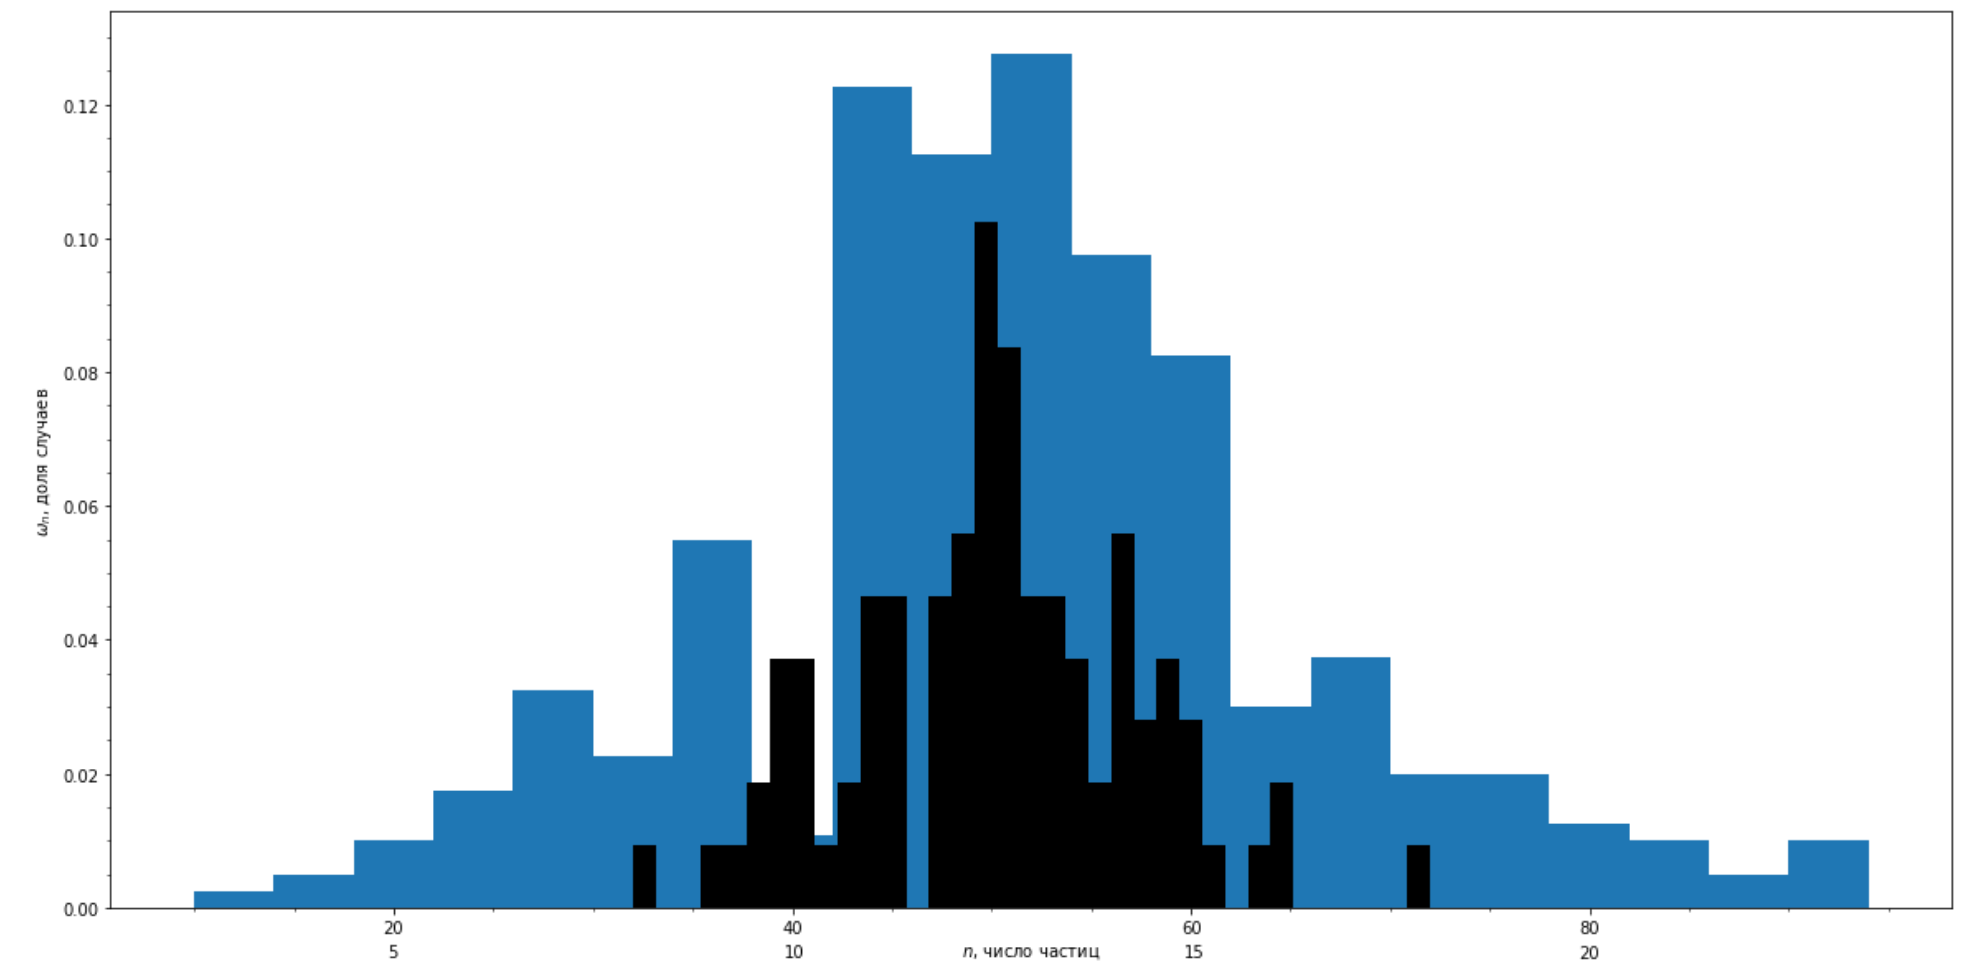
\includegraphics[scale = 0.56]{distribution.png}
			\caption{Гисторамма $\omega_n (n)$}
			\label{fig:my_label}
		\end{figure}
		\item Для обоих измерений определим среднее число частиц $\overline{n}$, среднеквадратичное отклонение отдельного измерения $\sigma_{отд}$ и среднего значения $\sigma_{\overline n}$:
		\[ \overline{n} = \frac{1}{N}\sum_{i=1}^N n_i, \:\:\:\:\: \sigma_{} = \sqrt{\frac{1}{N} \sum_{i=1}^{N}(n_i - \overline{n})^2}, \:\:\:\:\: \sigma_{\overline n} = \frac{1}{N} \sqrt{\sum_{i=1}^N(n_i - \overline n)^2} = \frac {\sigma_{}}{\sqrt{N}}, \] а также убедимся в справедливости формулы $\sigma_{} \approx \sqrt{\overline n}$.
		\par
		$t = 10 \: c$: $\overline n_1 = 12,53, \:\sigma_{1} = 3,47 ,\: \sigma_{\overline n_1} = 0,18$; $3.74 \approx \sqrt{14.09} = 3.75$.
		\par
		$t = 40 \: c$: $\overline n_2 = 50,11, \:\sigma_{2} = 7,15, \: \sigma_{\overline n_2} = 0,74$; $7,15 \approx \sqrt{50,11} = 7,08$.
		\item Найдём процент случаев, когда отклонение от среднего не превышает $\sigma, 2\sigma$. Сравним результаты с теоретическими оценками.
		\begin{center}
			\begin{tabular}{|c|c|c|}
				\hline
				Ошибка & Доля случаев, \% & Теоретическая оценка \\\hline
				$\sigma_1$ & 69 & 68\\\hline
				$2\sigma_1$ & 94,1 & 95\\\hline \hline
				$\sigma_2$ & 69 & 68\\\hline
				$2\sigma_2$ & 96,8 & 95\\\hline 
			\end{tabular}    
		\end{center}
		\item Наконец, найдём относительную погрешность средних значений:
		\[ \varepsilon_1 = \frac{1}{\sqrt{\overline{n_1}N_1}} = 1,46 \%, \:\:\: \varepsilon_2 = \frac{1}{\sqrt{\overline{n_2}N_2}} = 1,47 \%.\]
	\end{enumerate}
\section{Обсуждение результатов}
В ходе работы была произведена обработка данных в двух сериях экспериметов: с временем эксперимета 10 с и с временем эксперимета 40 с. Получены результаты соответственно $\overline n_1 = 12,53 \pm 0,18$ и    $\overline n_2 = 50,11 \pm 0,74$. Относительные погрешности определения $n_1$ и $n_2$ совпадают и весьма невелики ($1,46 \%$). Проверено, что результаты измерений соответствуют характерному для распределения Пуассона равенству: $\sigma = \sqrt{n_0}$.

\end{document}
	
	
	
	
	
	
	
	









